\chapter{Results}\label{chapter:results}

In this chapter I present how my CUDA solution compares against the TensorFlow implementations of $\Phi_{Flow}$.
\par All benchmarks were performed in a closed boundary environment with random divergence vectors in the $\left[-1, 1 \right]$ range. This may not represent real fluid simulations, since it is more expensive to compute with random vectors. However, as a benchmark it is well suited to compare the individual implementations. At the end of this chapter for comparison I present the average cg-iterations of a simple plume simulation.
\par The targeted residual accuracy was $1^{-5}$. Before starting the measurement, a warm-up of 5 runs was performed. The data shows the mean and standard deviation of 25 runs. The test system consists of a GeForce GTX 980, a Quad-Core Intel Core i7 3779K @3.5GHz CPU and 8GB of RAM.
\subsubsection{Performance Pressure Solve}
The following table shows the execution time per solve (t/s) and the average number of cg-iterations (iters) for quadratic grids and compares the TensorFlow solutions with my CUDA implementation: \\
\renewcommand{\arraystretch}{1.39}
\footnotesize
\begin{tabular}{l||l|l|l|l|l|l||r|r}
\hline
\multirow{2}{*}{Dimension} & \multicolumn{2}{l|}{TF CPU} & \multicolumn{2}{l|}{TF GPU} & \multicolumn{2}{l||}{CUDA} & \multirow{2}{*}{Speedup CPU} & \multirow{2}{*}{Speedup GPU} \\ \cline{2-7} 
                  & t/s        & iters        & t/s        & iters        & t/s         & iters        &             &             \\ \hline
$64^2$   & 49,65 ms &  & 108,2 ms &  & 25,36 ms &  & 2.0 x   & 4.2 x  \\ \hline
$128^2$  & 207,6 ms &  & 396,3 ms &  & 39,49 ms &  & 5.3 x   & 10.0 x \\ \hline
$256^2$  & 1,169 s  &   & 1,839 s &  & 77,19 ms &  & 15.1 x  & 23.8 x \\ \hline
$512^2$  & 12,75 s  &   & 12,90 s &  & 240,9 ms &  & 52.9 x  & 53.6 x \\ \hline
$1024^2$ & 133.7 s  &   & 87,47 s &  & 1,412 s  &  & 94.6 x  & 61.9 x \\ \hline
$2048^2$ & n/a      &   & n/a     &  & 9,742 s  &  & n/a     & n/a    \\ \hline \hline

$64^3$   & 3,878 s  &  & 2,473 s  &  & 42,18 ms &  & 91.9 x  & 58.6 x \\ \hline
$128^3$  & 55.22 s  &  & 29,35 s  &  & 397,1 ms &  & 139.1 x & 73.9 x \\ \hline
$256^3$  & n/a      &  & n/a      &  & 5,814 s  &  & n/a  & n/a 		  \\ \hline
\end{tabular}\\\\
\normalsize
Because of memory limitations on the test system, some tests could not be done in the TensorFlow implementations.

\begin{figure*}[t]
\centering
	\begin{subfigure}[b]{1\textwidth}
		\centering
		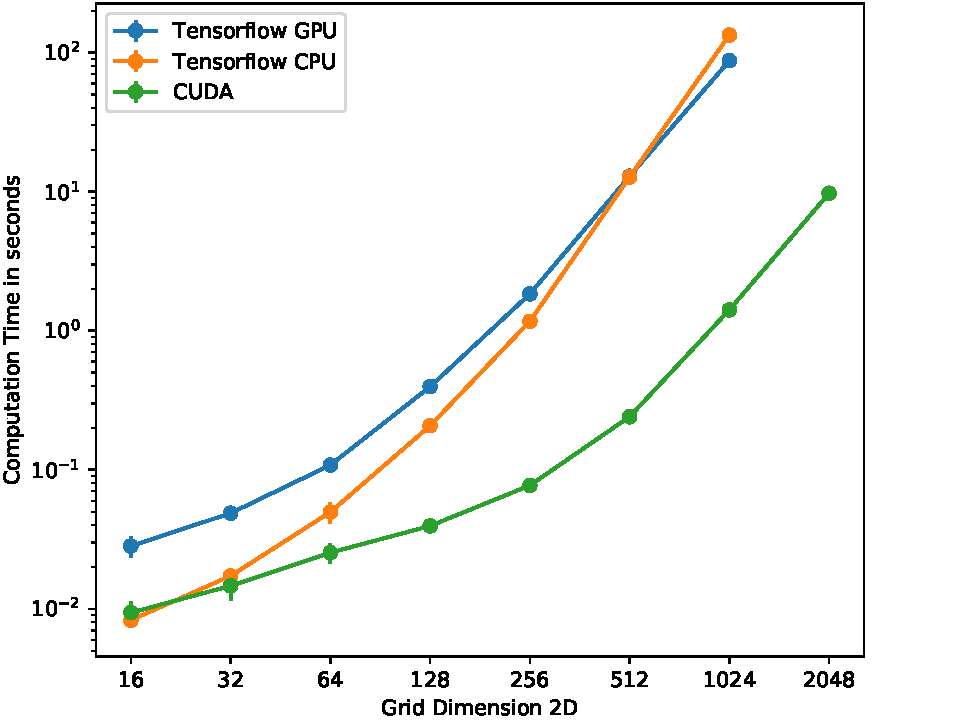
\includegraphics[height=9cm, width=14cm]{figures/2d_bs1}

		\caption{Pressure Solve in 2D}
	\end{subfigure}
	\begin{subfigure}[b]{1\textwidth}
		\centering
		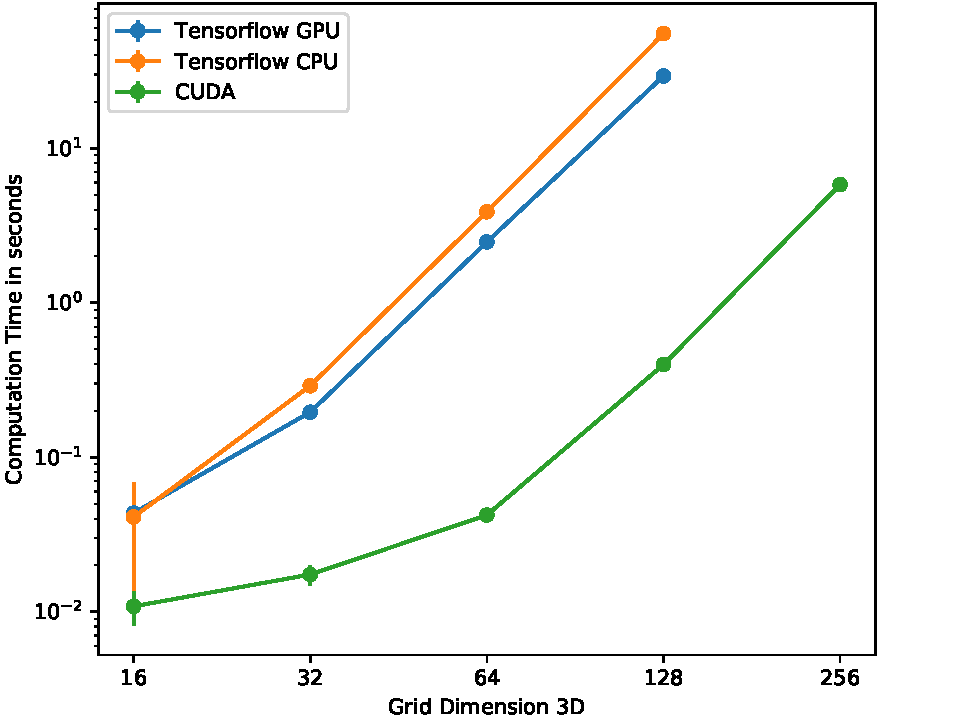
\includegraphics[height=9cm, width=14cm]{figures/3d_bs1}

		\caption{Pressure Solve in 3D}
	\end{subfigure}

\caption{Pressure Solve execution time with batch size 1.}	\label{fig:perfbs1}
\end{figure*}

\begin{figure*}[t]
\centering
	\begin{subfigure}[b]{1\textwidth}
		\centering
		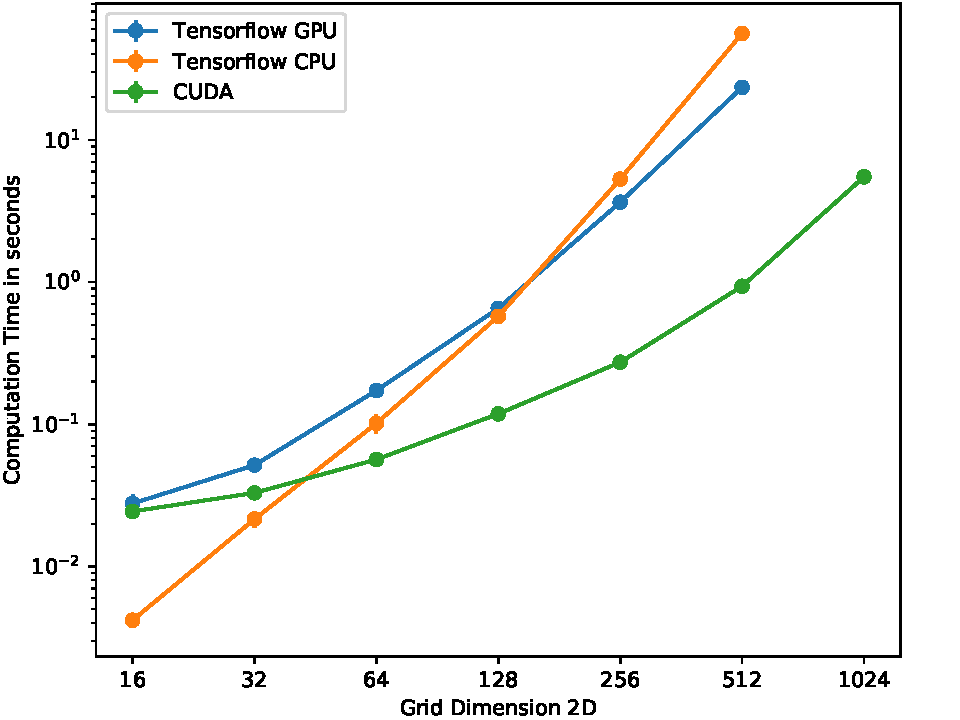
\includegraphics[height=9cm, width=14cm]{figures/2d_bs4}

		\caption{Pressure Solve in 2D}
	\end{subfigure}
	\begin{subfigure}[b]{1\textwidth}
		\centering
		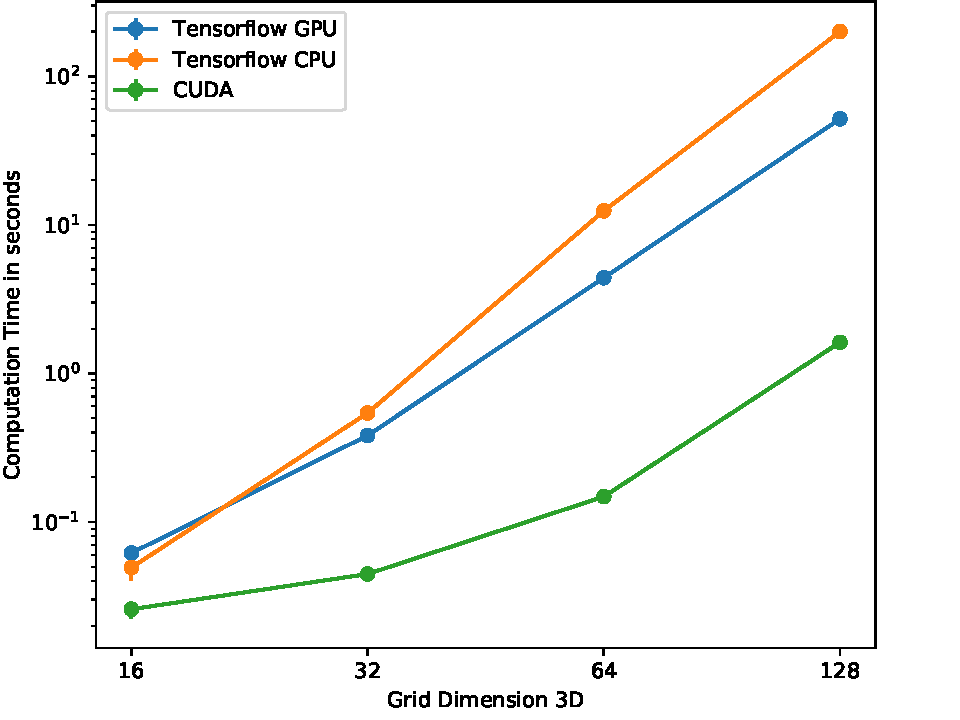
\includegraphics[height=9cm, width=14cm]{figures/3d_bs4}

		\caption{Pressure Solve in 3D}
	\end{subfigure}

\caption{Pressure Solve execution time with batch size 4.}	\label{fig:perfbs4}
\end{figure*}
\begin{figure*}[t]
\centering
	\begin{subfigure}[b]{1\textwidth}
		\centering
		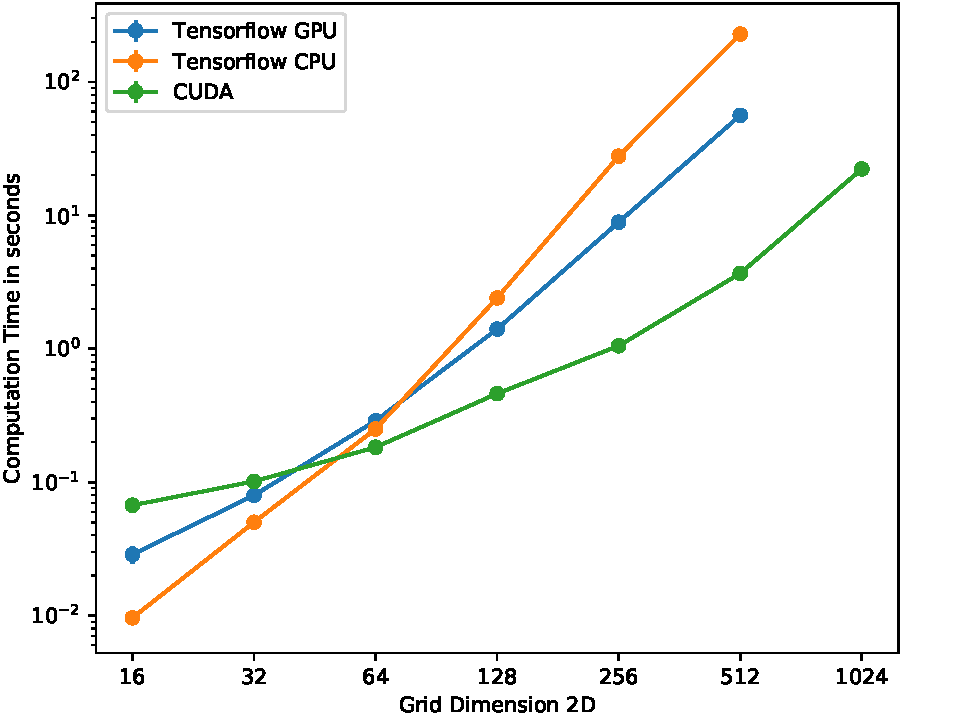
\includegraphics[height=9cm, width=14cm]{figures/2d_bs16}

		\caption{Pressure Solve in 2D}
	\end{subfigure}
	\begin{subfigure}[b]{1\textwidth}
		\centering
		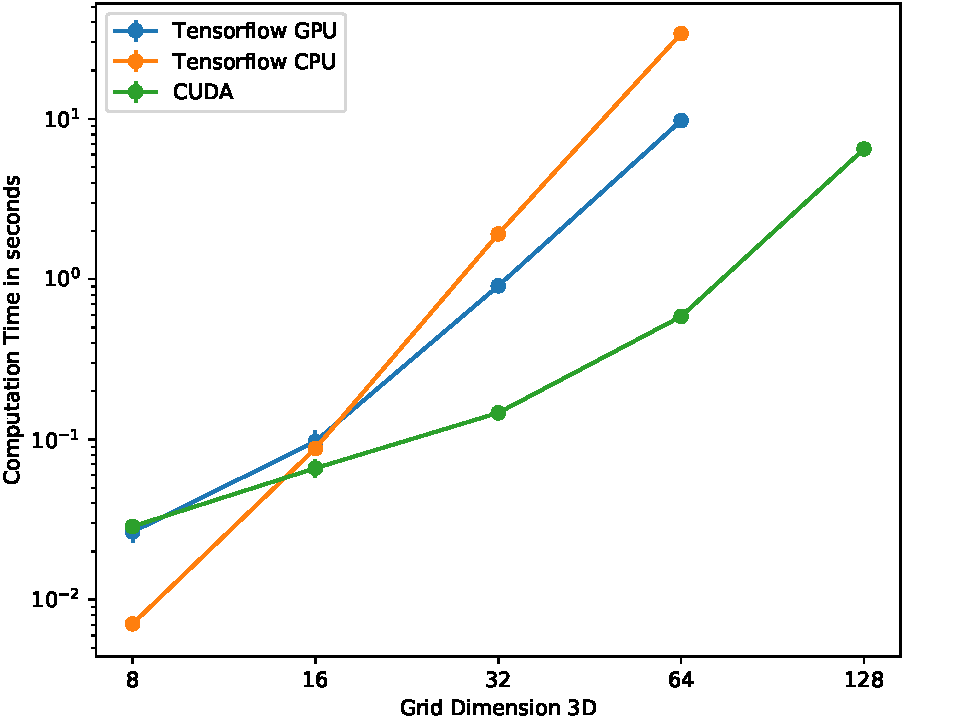
\includegraphics[height=9cm, width=14cm]{figures/3d_bs16}

		\caption{Pressure Solve in 3D}
	\end{subfigure}

\caption{Pressure Solve execution time with batch size 16.} \label{fig:perfbs16}
\end{figure*}


\clearpage
\subsubsection{Absolute and relative error}
\begin{figure*}[t]
\centering
	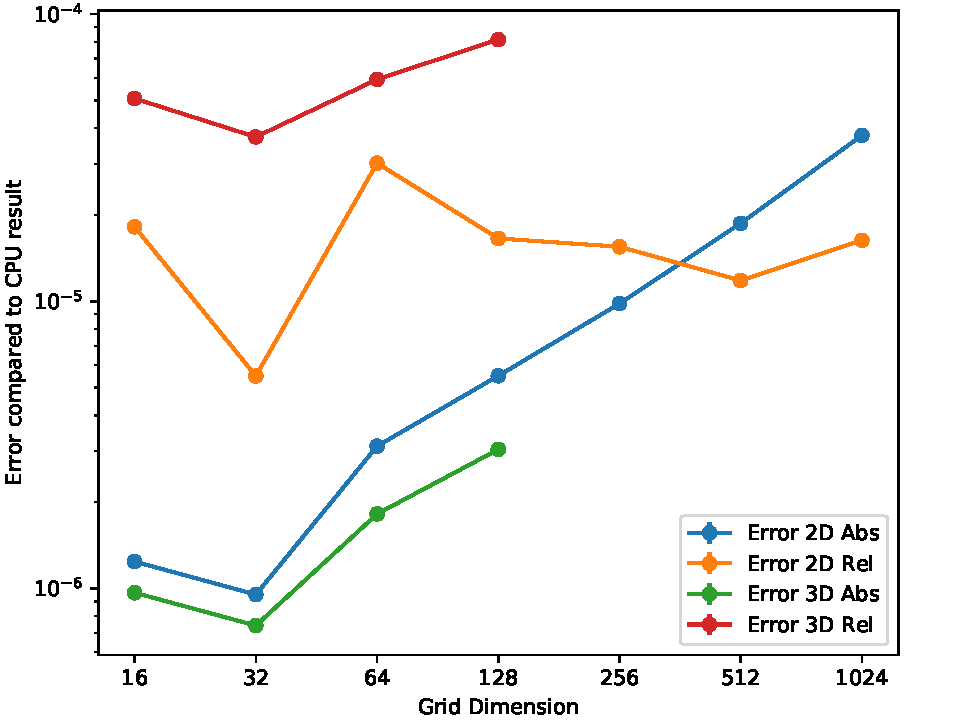
\includegraphics[height=9cm, width=14cm]{figures/error}
\caption{Absolute and relative error compared to the CPU version} \label{fig:error}
\end{figure*}
In this test, I compare how much my GPU solution differs from the CPU version of $\Phi_{Flow}$. I have calculated the absolute and relative difference between the pressure vectors component-wise. As stated in Fig. \ref{fig:error}, the error is sufficiently small.

\clearpage
\subsubsection{Performance Laplace Matrix generation}
The Speed of the Laplace Matrix generation is crucial for simulation with moving boundary conditions. $\Phi_{Flow}$ computes the Laplace Matrix once at startup on the CPU, so it does not infer with the simulation itself. Compared to the CPU implementation I could speed up the generation time up to a factor of 800 times. While the CPU version scales with the simulation size up, my parallelized CUDA implementation keeps constant significantly longer.


\begin{figure*}[t]
\centering
	\begin{subfigure}[b]{1\textwidth}
		\centering
		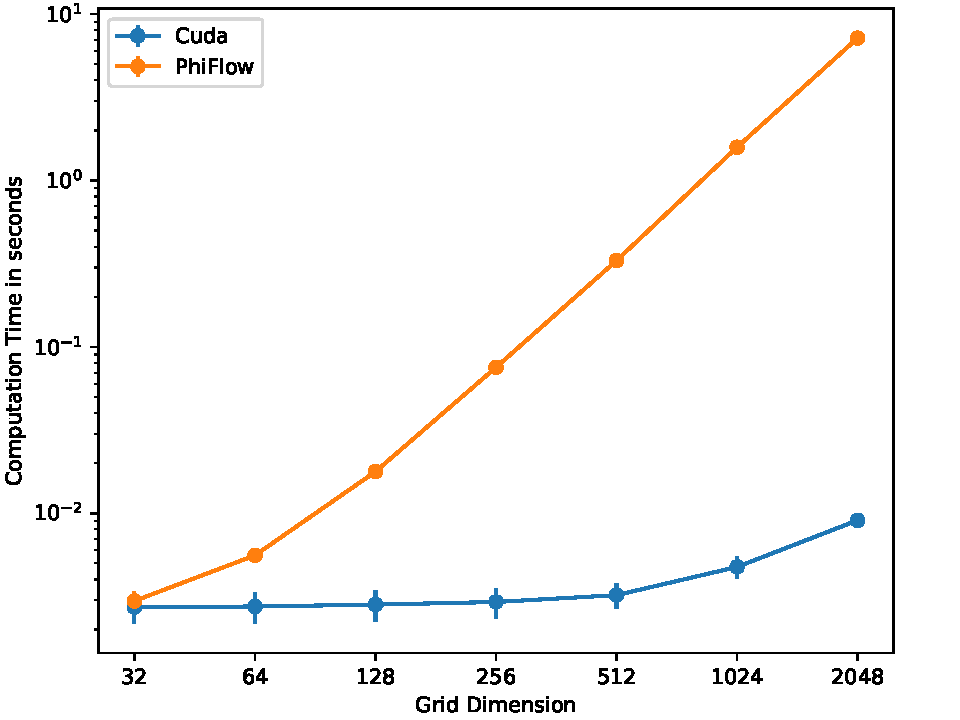
\includegraphics[height=9cm, width=14cm]{figures/laplace_2d}

		\caption{Laplace Matrix generation in 2D}
	\end{subfigure}
	\begin{subfigure}[b]{1\textwidth}
		\centering
		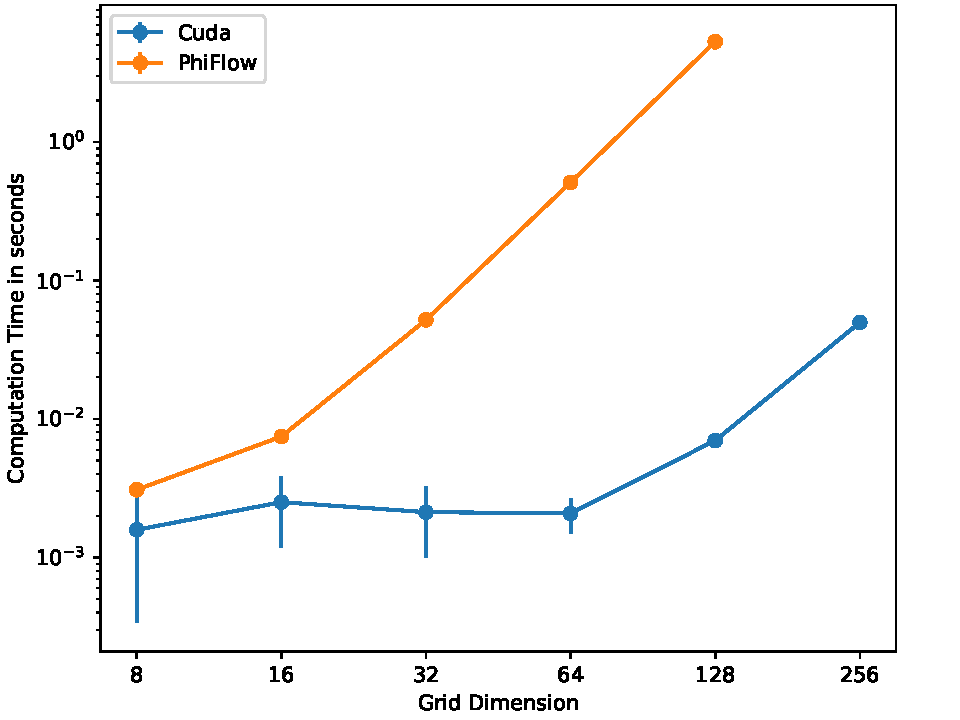
\includegraphics[height=9cm, width=14cm]{figures/laplace_3d}

		\caption{Laplace Matrix generation in 3D}
	\end{subfigure}

\caption{Laplace Matrix generation execution time} \label{fig:perfbs16}
\end{figure*}
